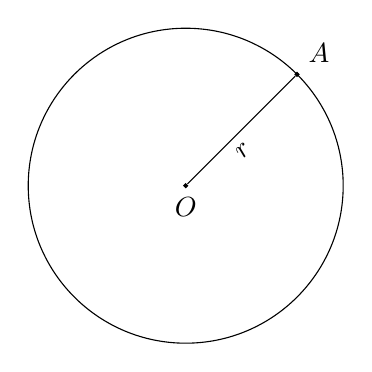
\begin{tikzpicture}
  [
    scale=2,
    >=stealth,
    point/.style = {draw, circle,  fill = black, inner sep = 0.5pt},
  ]
  \def\rad{1}
 \coordinate [point, label={below :	$O$ }] (O) at (0, 0);
  \draw (O) circle (\rad);  
    \node (A) at +(45:{\rad}) [point,label = above right:$A$ ] {};  
  \path
     (O)    edge  node[sloped, anchor=center, below, text width=0.5cm] { $r$}     (A) ; 
\end{tikzpicture}

